\subsection*{الف}
با $T=\frac{2\pi}{\omega_s}=\frac{2\pi}{3B}$:
\begin{flalign*}
s(t)&=\sum_{n=-\infty}^{\infty}\delta(t-nT)
\;\Longleftrightarrow\;
S(\omega)=\frac{2\pi}{T}\sum_{k=-\infty}^{\infty}\delta(\omega-3kB),\\
X(\omega)&=2\pi\delta(\omega)+\pi\bigl[\delta(\omega-B)+\delta(\omega+B)\bigr],\\
X_s(\omega)
&=\frac{1}{T}\sum_{k=-\infty}^{\infty}X(\omega-3kB)\\
&=\frac{2\pi}{T}\sum_k\delta(\omega-3kB)
+\frac{\pi}{T}\sum_k\!\left[
\delta\bigl(\omega-(3k+1)B\bigr)
+\delta\bigl(\omega-(3k-1)B\bigr)\right]. &&
\end{flalign*}

\begin{center}
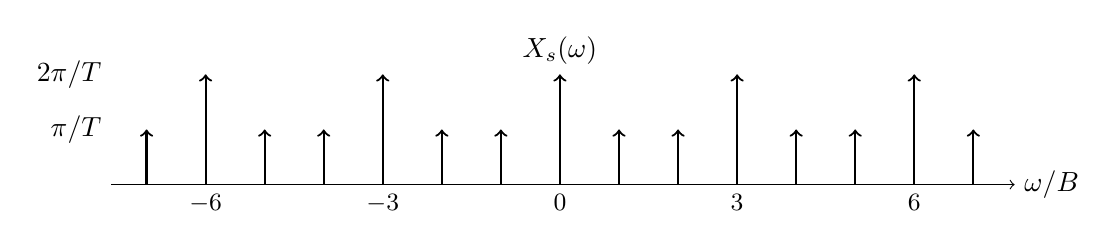
\begin{tikzpicture}[x=0.75cm,y=0.7cm]
\draw[->] (-7.6,0)--(7.7,0) node[right] {$\omega/B$};
\foreach \x in {-6,-3,0,3,6}
  \draw[->,thick] (\x,0)--(\x,2);
\foreach \x in {-7,-5,-4,-2,-1,1,2,4,5,7}
  \draw[->,thick] (\x,0)--(\x,1);
\foreach \x in {-6,-3,0,3,6}
  \node[below] at (\x,0) {\small $\x$};
\node[left] at (-7.6,2) {$2\pi/T$};
\node[left] at (-7.6,1) {$\pi/T$};
\node[above] at (0,2) {$X_s(\omega)$};
\end{tikzpicture}
\end{center}

\begin{flalign*}
H(\omega)&=
\begin{cases}
T,&|\omega|\le B,\\
\dfrac{T(3B-|\omega|)}{2B},&B<|\omega|<3B,\\
0,&|\omega|\ge3B,
\end{cases}\\
\widehat X(\omega)
&=H(\omega)X_s(\omega)\\
&=2\pi\delta(\omega)
+\pi\bigl[\delta(\omega-B)+\delta(\omega+B)\bigr]\\
&\quad+\frac{\pi}{2}
\bigl[\delta(\omega-2B)+\delta(\omega+2B)\bigr],\\
\widehat x(t)&=1+\cos(Bt)+\frac12\cos(2Bt). &&
\end{flalign*}

\begin{center}
\begin{tikzpicture}[x=1.2cm,y=0.9cm]
\draw[->] (-3,0)--(3,0) node[right] {$\omega/B$};
\draw[->,thick] (0,0)--(0,2);
\draw[->,thick] (-1,0)--(-1,1);
\draw[->,thick] (1,0)--(1,1);
\draw[->,thick] (-2,0)--(-2,0.5);
\draw[->,thick] (2,0)--(2,0.5);
\foreach \x in {-2,-1,0,1,2}
  \node[below] at (\x,0) {\small $\x$};
\node[left] at (-3,2) {$2\pi$};
\node[left] at (-3,1) {$\pi$};
\node[left] at (-3,0.5) {$\pi/2$};
\node[above] at (0,2) {$\widehat X(\omega)$};
\end{tikzpicture}
\end{center}

\subsection*{ب}
هیچ مؤلفه‌ای از $X(\omega)$ حذف نشده است، زیرا
\begin{flalign*}
\omega_s=3B>2B,\qquad
H(0)=H(\pm B)=T. &&
\end{flalign*}
پس اتلاف اطلاعات نداریم؛ ولی به علت عبور تصویرهای $\omega=\pm2B$، بازسازی اعوجاج دارد و $\widehat x(t)\ne x(t)$.

\subsection*{ج}
شرط قسمت قبل برقرار نیست. با این حال، برای بازسازی دقیق با همین $H(\omega)$ باید نزدیک‌ترین تصویر نیز خارج از ناحیهٔ عبور فیلتر باشد:
\begin{flalign*}
\omega_s-B\ge3B
\quad\Longrightarrow\quad
\boxed{\omega_s\ge4B}. &&
\end{flalign*}

\textbf{پاسخ دیگر}

\subsection*{الف}
طیف سیگنال اصلی و سیگنال نمونه‌برداری‌شده:
\begin{flalign*}
X(\omega) &= 2\pi \delta(\omega) + \pi \delta(\omega - B) + \pi \delta(\omega + B) && \
X_s(\omega) &= \frac{1}{T} \sum_{k=-\infty}^{\infty} X(\omega - k\omega_s) = \frac{1}{T} \sum_{k=-\infty}^{\infty} X(\omega - 3kB) &&
\end{flalign*}
با عبور از فیلتر بازسازی، طیف خروجی $\hat{X}(\omega) = X_s(\omega)H(\omega)$ با توجه به مقادیر فیلتر ($H(0) = T$، $H(\pm B) = T$ و $H(\pm 2B) = T/2$) به دست می‌آید:

\begin{center}
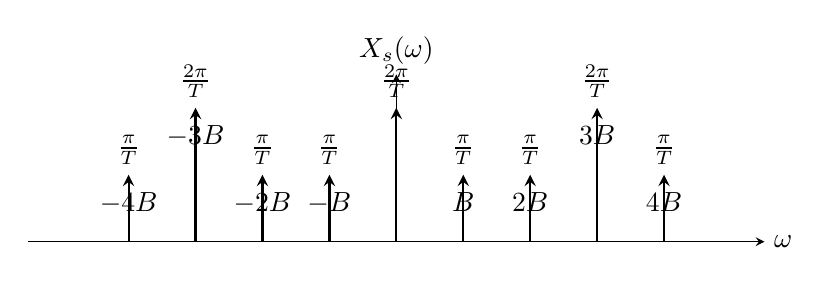
\begin{tikzpicture}[scale=0.85, >=stealth]
\draw[->] (-5.5,0) -- (5.5,0) node[right] {$\omega$};
\draw[->] (0,0) -- (0,2.5) node[above] {$X_s(\omega)$};
\draw[->, thick] (0,0) -- (0,2) node[above] {$\frac{2\pi}{T}$};
\draw[->, thick] (1,0) -- (1,1) node[above] {$\frac{\pi}{T}$} node[below, yshift=-0.1cm] {$B$};
\draw[->, thick] (2,0) -- (2,1) node[above] {$\frac{\pi}{T}$} node[below, yshift=-0.1cm] {$2B$};
\draw[->, thick] (3,0) -- (3,2) node[above] {$\frac{2\pi}{T}$} node[below, yshift=-0.1cm] {$3B$};
\draw[->, thick] (4,0) -- (4,1) node[above] {$\frac{\pi}{T}$} node[below, yshift=-0.1cm] {$4B$};
\draw[->, thick] (-1,0) -- (-1,1) node[above] {$\frac{\pi}{T}$} node[below, yshift=-0.1cm] {$-B$};
\draw[->, thick] (-2,0) -- (-2,1) node[above] {$\frac{\pi}{T}$} node[below, yshift=-0.1cm] {$-2B$};
\draw[->, thick] (-3,0) -- (-3,2) node[above] {$\frac{2\pi}{T}$} node[below, yshift=-0.1cm] {$-3B$};
\draw[->, thick] (-4,0) -- (-4,1) node[above] {$\frac{\pi}{T}$} node[below, yshift=-0.1cm] {$-4B$};
\end{tikzpicture}

\vspace{0.5cm}

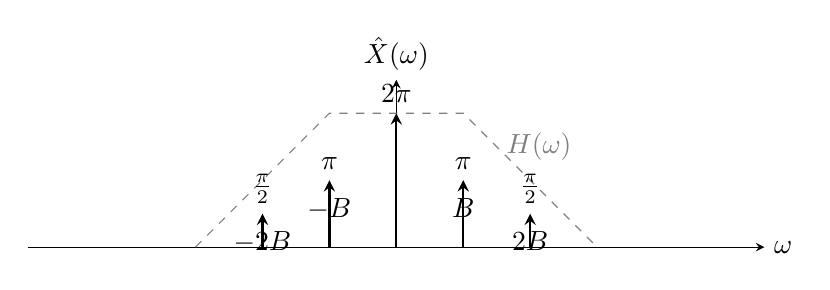
\begin{tikzpicture}[scale=0.85, >=stealth]
\draw[->] (-5.5,0) -- (5.5,0) node[right] {$\omega$};
\draw[->] (0,0) -- (0,2.5) node[above] {$\hat{X}(\omega)$};
\draw[dashed, gray] (-3,0) -- (-1,2) -- (1,2) -- (3,0);
\node[gray, right] at (1.5,1.5) {$H(\omega)$};
\draw[->, thick] (0,0) -- (0,2) node[above] {$2\pi$};
\draw[->, thick] (1,0) -- (1,1) node[above] {$\pi$} node[below, yshift=-0.1cm] {$B$};
\draw[->, thick] (2,0) -- (2,0.5) node[above] {$\frac{\pi}{2}$} node[below, yshift=-0.1cm] {$2B$};
\draw[->, thick] (-1,0) -- (-1,1) node[above] {$\pi$} node[below, yshift=-0.1cm] {$-B$};
\draw[->, thick] (-2,0) -- (-2,0.5) node[above] {$\frac{\pi}{2}$} node[below, yshift=-0.1cm] {$-2B$};
\end{tikzpicture}
\end{center}

\subsection*{ب}
بله، سیگنال به درستی بازیابی نمی‌شود و دچار اعوجاج می‌گردد:
\begin{flalign*}
\hat{X}(\omega) &= 2\pi \delta(\omega) + \pi \delta(\omega - B) + \pi \delta(\omega + B) + \frac{\pi}{2} \delta(\omega - 2B) + \frac{\pi}{2} \delta(\omega + 2B) && \
\implies \hat{x}(t) &= 1 + \cos(Bt) + \frac{1}{2}\cos(2Bt) \neq x(t) &&
\end{flalign*}
دلیل: فیلتر $H(\omega)$ ایده‌آل نیست و مؤلفه‌های فرکانسی $\pm 2B$ از کپی اول طیف (در $\omega_s = \pm 3B$) را کاملاً حذف نمی‌کند.

\subsection*{ج}
برای جلوگیری از پدیدهٔ \lr{Aliasing} در خروجی فیلتر، پایین‌ترین فرکانسِ کپی‌های طیفی باید خارج از باند غیرصفر فیلتر (یعنی محدودهٔ فرکانسی تا $3B$) قرار گیرد:
\begin{flalign*}
\omega_s - \omega_m \geq 3B \implies \omega_s - B \geq 3B \implies \omega_s \geq 4B &&
\end{flalign*}